\documentclass{article}

%\VignetteEngine{knitr::knitr}
%\VignetteIndexEntry{edge Package}


\usepackage{graphics}
\usepackage{amsmath}
\usepackage{fullpage}
\usepackage{bibentry}
\usepackage[section]{placeins}
\usepackage[round]{natbib}
\usepackage{authblk}
\usepackage[parfill]{parskip}
\setlength{\parskip}{10pt}
%\usepackage{indentfirst}
\usepackage[colorlinks=true]{hyperref}
\usepackage[utf8]{inputenc}
\nobibliography*



\usepackage{Sweave}
\begin{document}
\Sconcordance{concordance:edge.tex:edge.Rnw:%
1 21 1 46 0 1 5 37 1 4 0 22 1 6 0 3 1 1 9 %
17 1 5 0 23 1 4 0 7 1 5 0 7 1 4 0 15 1 4 0 %
10 1 4 0 37 1 4 0 8 1 4 0 7 1 6 0 7 1 35 0 %
19 1 6 0 11 1 6 0 7 1 26 0 17 1 4 0 12 1 6 %
0 7 1 6 0 7 1 26 0 16 1}



\title{{\tt edge}:\\ Extraction of Differential Gene Expression \\ Version 0.99.0}

\author[1]{John D. Storey\thanks{\url{http://genomine.org/contact.html}}}
\author[2]{Jeffrey T. Leek}
\author[1]{Andrew J. Bass}
\affil[1]{Princeton University}
\affil[2]{John Hopkins University}

\renewcommand\Authands{ and }

\maketitle
\tableofcontents
\newpage
\section{Introduction}

{\tt edge} is a package for significance analysis of DNA micro-array experiments and is able to identify genes that are differentially expressed between two or more different biological conditions (e.g., healthy versus diseased tissue). {\tt edge} performs significance analysis by using a new method developed by \cite{storey:2007} called the optimal discovery procedure (ODP). Whereas previously existing methods employ statistics that are essentially designed for testing one gene at a time (e.g., t-statistics and F-statistics), the odp-statistic uses information across all genes to test for differential expression. \cite{storey:etal:2007} shows that the ODP is a more intuitive, often times more powerful, approach to multiple hypothesis testing problems when compared to traditional methods. 

%\texttt{edge} provides methods, detailed in \cite{storey:2005}, that have been specifically designed for time course experiments because many things can go wrong when using traditional methods designed for static experiments. Even though some significance analysis packages allow for users to enter information about time points, a rigorously developed set of methodology that simplifies the process for time course experiments is available in {\tt edge}. 

The improvements in power are substantial; Figure 1 shows a comparison between edge and five leading software packages, based on the \cite{hedenfalk:2001} breast cancer expression study. In addition to identifying differentially expressed genes, {\tt edge} includes implementations of popular packages such as {\tt snm} and {\tt sva}.  

\begin{figure}[ht]
\begin{center}
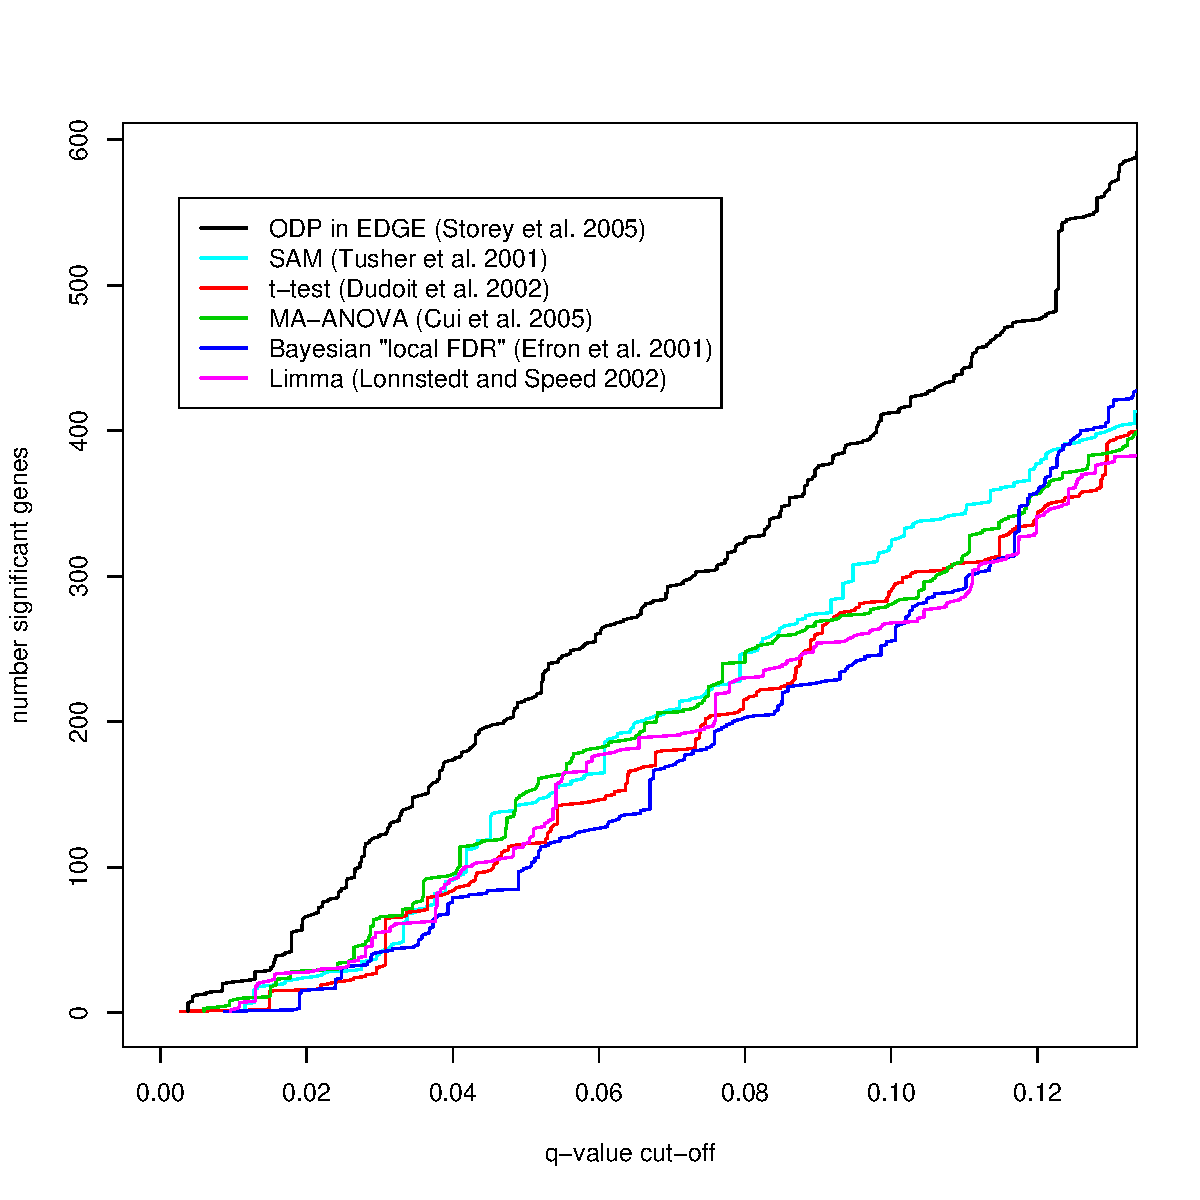
\includegraphics[scale=.50]{edgecomp.pdf}
\end{center}
\caption{Comparison of EDGE to various other leading methods for identifying differential expressed genes in the \cite{hedenfalk:2001} study. Figure is from \cite{leek2005}.}
\label{fig:test}
\end{figure}

%There are three experimental designs where {\tt edge} can identify differentially expressed genes: static, time course and continuous response experiments. In a ``static sampling'' experiment, the arrays have been collected from distinct biological groups without respect to time. The goal is to identify genes that have a statistically significant difference in average expression across these distinct biological groups. The second type of experiment is a time course experiment, where the arrays have been sampled with respect to time from one or more distinct biological groups. If only one biological group has been sampled, then the goal is to identify genes that show ``within-class temporal differential expression'', i.e., genes that show statistically significant changes in expression over time. If two or more biological groups have been sampled, then the goal is to identify genes that show ``between-class temporal differential expression'', i.e., genes that show statistically significant differences in expression over time between the various groups. The third type of experiment is a ``continuous response'' design, which means that the arrays have been collected from a continuously defined biological state without respect to time. The goal here is to identify genes whose expression shows a statistically significant change with respect to this continuous response.

\section{Citing this package}

\textbf{[1] \bibentry{storey:2007}} \\
Theory paper that introduces the optimal discovery procedure and shows that it maximizes the expected true postive results for each number of fixed false positive results. The optimality is closely related to the false discovery rate.

\textbf{[2] \bibentry{storey:etal:2007}} \\
Dicusses various ways of estimating the ODP statistic with applications to microarray experiments.

\textbf{[3] \bibentry{woo:leek:storey:2011}} \\
Previous implementations of the ODP are computationally infeasible for a large number of hypothesis tests. This paper introduces a computationally efficient implementation of ODP that this package is based on.

\section{Getting help}
Hopefully, most questions relating to the package will be answered in the vignette but to get a more detailed account of how to use the functions simply type within R:
\begin{Schunk}
\begin{Sinput}
> help(package="edge")
\end{Sinput}
\end{Schunk}
\noindent Please contact the authors directly with any issues regarding bugs. Otherwise, any questions or problems implementing {\tt edge} will most efficiently be addressed on the Bioconductor mailing list, \url{http://stat.ethz.ch/mailman/listinfo/bioconductor}.

\section{Quick start guide}
To get started, first load the {\tt kidney} dataset included in the package: 
\begin{Schunk}
\begin{Sinput}
> library(edge)
> data(kidney)
> kidexpr <- kidney$kidexpr
> age <- kidney$age
> sex <- kidney$sex
\end{Sinput}
\end{Schunk}
The {\tt kidney} study is interested in determining differentially expressed genes in the kidney as it ages. The {\tt age} variable is the age of the subjects and the {\tt sex} variable is whether the subjects were male or female. The expression values for the genes are contained in the {\tt kidexpr} variable which is a 1500 by 72 matrix (a small subset of the real dataset).

Once the data has been loaded, the user has two options to create an {\tt edgeSet} object: {\tt edgeModel} or {\tt edgeStudy}. If the experiment models are unknown to the user, {\tt edgeStudy} can be used to create the models:
\begin{Schunk}
\begin{Sinput}
> edgeObj <- edgeStudy(data = kidexpr, adj.var = sex, tme = age, sampling = "timecourse")